\section{Aufbau und Durchf"uhrung}
\label{sec:durchfuehrung}
	Der Versuch wird, wie in nachfolgender Abbildung dargestellt, aufgebaut.
	Die Ladung $Q$ wird "uber einen Widerstand $R$ auf einem Kondensator $C$ gesammelt und durch einen Verst"arker in den Z"ahler geleitet.
	Zudem l"asst sich jeder Impuls im Oszilloskop sichtbar machen, was die Identifizierung von Nachentladungen erm"oglicht.

	Die angelegte Spannung kann variiert werden, um die Z"ahlrohrcharakteristik aufnehmen zu k"onnen.

	\begin{figure}[h]
		\centering
		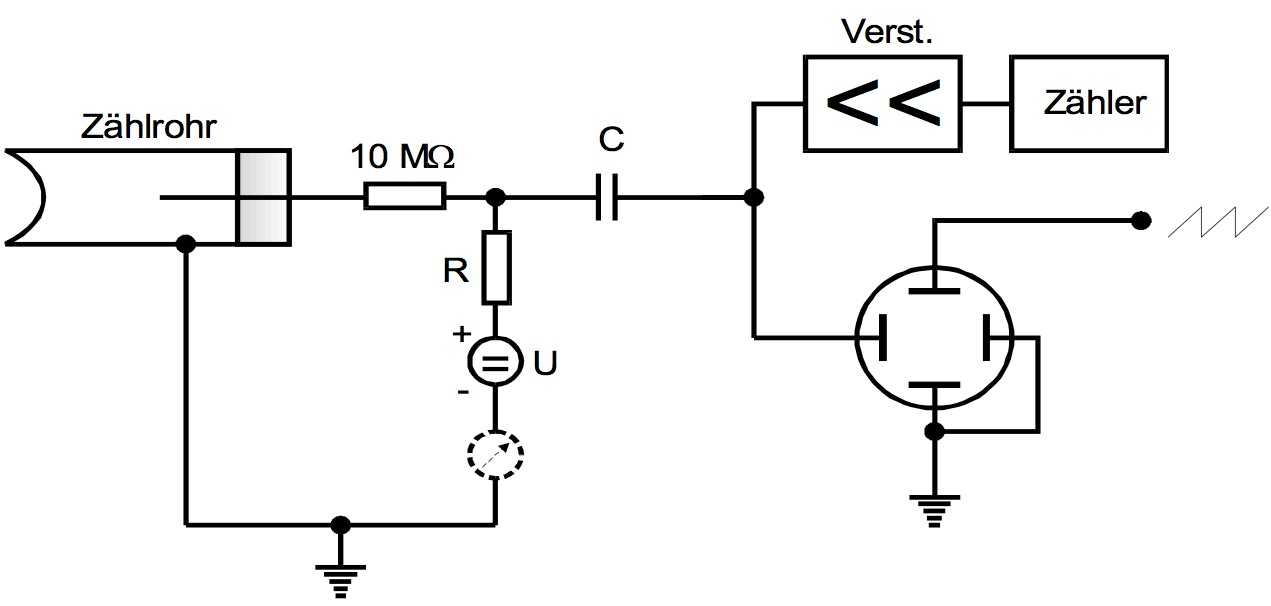
\includegraphics[width = 15cm]{img/aufbau.jpeg}
		\caption{Versuchsaufbau \cite{anleitung}}
		\label{fig:aufbau}
	\end{figure}

	\subsection{Messungen}
	\label{subsec:messungen}
		Zun"achst wird die Z"ahlrate $N$ in Abh"angigkeit der Spannung $U$ aufgenommen, um die Charakteristik des Geiger-M"uller-Z"ahlrohrs zu bestimmen.
		Auf Grund der Totzeit muss darauf geachtet werden, dass die Z"ahlrate im einzelnen nicht $N = \SI{100}{\per \second}$ "ubersteigt.
		Der Fehler $\Delta N$ der Messungen soll dabei unter $\Delta N = \SI{1}{\percent}$ liegen.
		Weil die Werte poissonverteilt sind, gilt

		\begin{eqnarray*}
			\Delta N = \sqrt{N} & < & \SI{.01}{} \\
			\Rightarrow \quad N & > & \SI{10000}{} \, .
		\end{eqnarray*}

		Anschlie"send sollen die Nachentladungen sichtbar gemacht werden.
		Die Strahlintensit"at muss daf"ur so gering sein, dass praktisch jeder einzelne Strahlungsimpuls sichtbar ist und Nachentladungen zun"achst ausgeschlossen werden k"onnen.
		Daf"ur wird die Spannung $U$ auf einen Wert am Anfang des Plateaus eingestellt.
		Sobald einzelne Impulse nachgewiesen werden, wird die Spannung $U$ maximal eingestellt und die Impulse der Nachentladung werden sichtbar.
		Hierbei ist der zeitliche Abstand $T_\mathrm{tot}$ zwischen Prim"ar- und Nachentladungsimpuls vom Oszilloskop abzulesen.


		Die Totzeit $T_\mathrm{tot}$ soll zudem mit Hilfe der Zwei-Quellen-Methode gemessen werden.
		Hierf"ur wird die Z"ahlrate $N_1$ zun"achst f"ur eine Quelle gemessen.
		Ohne die Quelle zu ver"andern, wird eine weitere Quelle hinzugef"ugt und wiederum $N_{1+2}$ gemessen.
		Die erste Quelle wrid dann entfernt und es wird ein letztes Mal $N_2$ gemessen.

		Die Werte zeigen dann, dass auf Grund der Totzeit $T_\mathrm{tot}$ n"aherungsweise gilt: 

		\begin{eqnarray}
			N_{1+2} & < & N_1 + N_2 \nonumber \\
			\Rightarrow \quad T_\mathrm{tot} & \approx & \frac{N_1 + N_2 - N_{1+2}}{2 N_1 N_2} \label{totzeit} \,.
		\end{eqnarray}


		Schlie"slich wird die pro Teilchen freigesetzte Ladungsmenge $Q$ in Abh"angigkeit von der Spannung $U$ ermittelt.
		Hierf"ur wird der mittlere Z"ahlstrom $\overline{I}$ gemessen.